\documentclass[10pt]{beamer}

\usepackage[T2A]{fontenc}
\usepackage[utf8]{inputenc}
\usepackage[russian,english]{babel}

\usefonttheme[onlymath]{serif}

\usetheme[progressbar=frametitle]{metropolis}
\usepackage{appendixnumberbeamer}

\usepackage{booktabs}
\usepackage[scale=2]{ccicons}

\usepackage{pgfplots}
\usepgfplotslibrary{dateplot}

\usepackage{xspace}
\newcommand{\themename}{\textbf{\textsc{metropolis}}\xspace}
\newcommand{\TODO}[1]{\textbf{\textcolor{red}{TODO: #1}}}

\date{}
\author{Екатерина Тузова}


\title{Лекция 5}
\subtitle{Байесовские методы классификации}

\begin{document}

\section{Разбор летучки}

\maketitle

\begin{frame}{}
	\centering
	\begin{figure}
		\begin{minipage}{.5\textwidth}
		  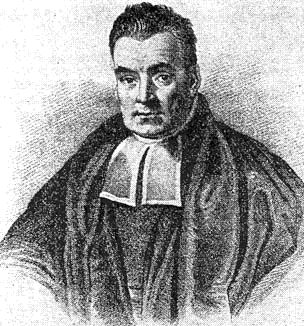
\includegraphics[width=0.9 \linewidth, height=150pt, keepaspectratio]{images/bayes}
		\end{minipage}%
		\begin{minipage}{.5\textwidth}				
			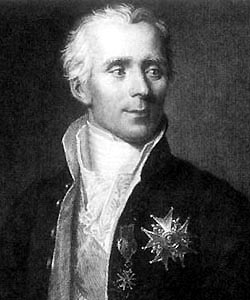
\includegraphics[width=0.9 \linewidth, height=150pt, keepaspectratio]{images/laplace}
		\end{minipage}
	\end{figure}
\end{frame}

\section{Мотивирующий пример}

{\foot{\href{http://qwone.com/~jason/20Newsgroups}{http://qwone.com/~jason/20Newsgroups}}
\begin{frame} {Классификация сообщений}
  Датасет \alert{20 newsgroups} содержит почти 20000 сообщений из списков рассылки Usenet.\\
  \pause
  \bigbreak
  Примеры сообщений из списка рассылки sci.crypt:\\
  \begin{quotation}
    When you find out a floppy password protect program, could you e-mail me.\\
    Thanks\\
    \bigbreak
    Not to mention Computer Associates. I'll have to be careful to stop telling people I'm a Clipper programmer, they might lynch me... :-)
  \end{quotation}
  \pause
  \alert{Задача}: Построить классификатор, предсказывающий по тексту сообщения список рассылки, в который оно было отправлено.
\end{frame}
}

{\foot{a priori, likelihood}
\begin{frame} {Вероятностная постановка задачи}
  $X$ -- множество объектов\\
  $Y$ -- множество меток классов\\
  $X \times Y$ -- вероятностное пространство с плотностью \\
  $$p(x,y) = P_yp(x|y)$$\\
  \bigbreak
  $P_y$ -- априорная вероятность класса $y$\\
  $p(x|y)$ -- функция правдоподобия класса $y$\\
  \bigbreak
  \pause
  \alert{Задача}: Построить алгоритм $a: X \rightarrow Y$, минимизирующий \textbf{вероятность} ошибки.
\end{frame}
}

\begin{frame} {Плотности $p(x|y)$}
  \centering
  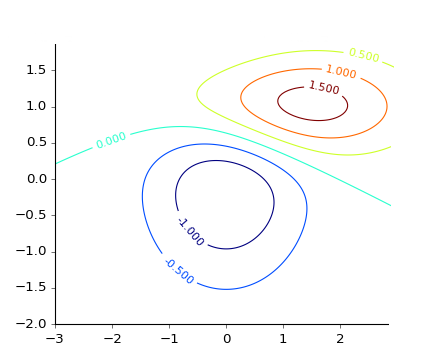
\includegraphics[width=0.9 \textwidth, height=0.9 \textheight, keepaspectratio]{images/density}
\end{frame}

\begin{frame}{Известное и неизвестное}
  Как правило, априорные вероятности $P_y$ и функции правдоподобия классов $p(x|y)$ неизвестны.\\
  \pause
  \bigbreak
  2 подзадачи:
  \begin{enumerate}
    \item По выборке $X^l$ из неизвестного распределения с плотностью $p(x, y)$ построить оценки вероятностей $\hat{P}_y$ и функций правдоподобия $\hat{p}(x|y)$ для каждого класса
    \item По известным $P_y$ и $p(x|y)$ построить функцию $a(x)$, минимизирующую вероятность ошибочной классификации
  \end{enumerate}
\end{frame}

\begin{frame}{Вопрос}
  \centering
  Предположим, что нам известно заранее распределение с плотностью $p(x, y)$. Как оценить вероятность ошибочной классификации для произвольного алгоритма $a: X \rightarrow Y$?
\end{frame}

\begin{frame}{Функционал среднего риска}
  $a: X \rightarrow Y$ разбивает $X$ на непересекающиеся области:\\
  $$A_s = \{x \in X | a(x) = s \} \quad s \in Y $$\\
  \bigbreak 
  \pause
  \alert{Ошибка}: объект $x$ класса $y$ попадает в $A_s$, $s \neq y$\\
  \bigbreak
  Вероятность ошибки: $p(A_s, y) = \int\limits_{A_s} p(x, y) dx$
\end{frame}

\begin{frame}{Функционал среднего риска}
  \alert{Идея}: Введем $\lambda_{y}$ -- штраф за назначение неправильного класса объекту из $y$\\
  \pause
  \bigbreak
  Функционал среднего риска алгоритма $a$:\\
  $$R(a) = \sum\limits_{s \in Y} \sum\limits_{y \in Y} \lambda_{y} P_y p(A_s|y)$$\\
%  \bigbreak
%  $\lambda_{y} = \left[ y \neq s \right]$, то $R(a)$ -- вероятность ошибки алгоритма $a(x)$
\end{frame}

{\foot{Optimal Bayes Classifier}
\begin{frame}{Оптимальный Байесовский классификатор}
  Минимум среднего риска $R(a)$ достигается при:\\
  $$a(x) = \arg\max\limits_{y \in Y} \lambda_y P_y p(x|y)$$
\end{frame}
}

{\foot{Maximum a posteriori estimation}
\begin{frame}{Принцип максимума апостериорной вероятности}
  Апостериорная вероятность класса $y$ для объекта $x$:
      $$
    P(y|x)
    = \dfrac{p(x, y)}{p(x)}
    = \dfrac{P_y p(x|y)}{\sum\limits_{s \in Y} P_s p(x|s)}
    \propto P_y p(x|y)
    $$
  \pause
  Перепишем оптимальный алгоритм с использованием апостериорных вероятностей:\\
  $$a(x) = \arg\max\limits_{y \in Y} \lambda_y P(y|x)$$\\
  \bigbreak
  Если $\lambda_y = 1$, то алгоритм максимизирует апостериорную вероятность для объекта $x$.
\end{frame}
}

\begin{frame}{Вопрос}
  \centering
  Чего еще не хватает для \alert{работающего} классификатора?
\end{frame}

\begin{frame} {На полпути к классификатору}
  \begin{enumerate} [<+->]
    \item Что представляют из себя $X$ и $Y$ для сообщений из списков рассылки
    \item Выбрать функции правдоподобия $p(x|y)$
    \item Научиться оценивать априорные вероятности классов $\hat{P}_y$ и функции правдоподобия $\hat{p}(x|y)$ из данных
  \end{enumerate}
\end{frame}

\begin{frame}{Векторизация с использованием словаря}
  $V = {v_1, \dots, v_{|V|}}$ -- упорядоченное множество слов\\
  \bigbreak
  Сообщение можно представить в виде вектора, в котором на $j$-ой позиции стоит $1$, если $v_d$ встречается в сообщении, и $0$ в противном случае\\
  \bigbreak
  $X\equiv \{0, 1\}^{|V|}$ , а $Y$ это множество идентификаторов рассылки
\end{frame}

\begin{frame}{Пример}
  V = {who, I, let, dogs, out, the}\\
  \pause
  \bigbreak
  Сообщение «Who let the dogs out? Who, who, who, who?» будет векторизовано как [1, 0, 1, 1, 1, 1].\\
  \pause
  \bigbreak
  Как будет векторизовано предложение «Well, if I am a dog, the party is on [...]»?
\end{frame}

\begin{frame}{Функция правдоподобия}
  \centering 
  Как определить функцию правдоподобия для сообщения, представленного в виде бинарного вектора?
\end{frame}

\section{Наивность}

\begin{frame} {Функция правдоподобия}
  \alert{Идея}: будем использовать дискретное распределение на множестве $X$, то есть сопоставим вероятность $\theta_{yx}$ каждому
значению $x \in X$, тогда\\
$$p(x|y) = \theta_{yx}$$
\end{frame}

\begin{frame} {Функция правдоподобия}
  \alert{Идея}: Предположим, что все признаки (компоненты вектора $x$) независимы \alert{при условии} $y$, тогда:\\
  $$p(x|y) = \prod\limits_{d=1}^{|V|} p(x^d | y)$$\\
  \pause
  \bigbreak
  Полученный классификатор называют \alert{наивным} Байесовским классификатором из-за наивности сделанного предположения\\
  $$a(x) = \arg\max_{y \in Y} \lambda_y P_y \prod\limits_{d=1}^{|V|} p(x^d | y)$$
\end{frame}

{\foot{Daniel Bernoulli}
\begin{frame} {Распределение Бернулли}
  Распределение Бернулли -- дискретное распределение на множестве ${0, 1}$ с параметром $\theta \in [0, 1]$ — вероятностью \alert{успеха} и функцией вероятности:\\
  $$Ber(x; \theta) = \theta^x (1 - \theta)^{1-x}$$
  \bigbreak
  \pause
  $$p(x|y) = \prod\limits_{d=1}^{|V|} \theta_{yd}^x (1 - \theta_{yd})^{1-x}$$\\

\end{frame}
}

{\foot{maximum likelihood estimation}
\begin{frame}{Метод максимального правдоподобия}
  Попробуем оценить параметры функций правдоподобия по выборке $X^l$.\\
  $$L(\theta) = \sum\limits_{i=1}^{l} \ln p(x_i;\theta) \rightarrow \max\limits_{\theta}$$
  Как записать условие оптимума?
\end{frame}
}

\begin{frame}{Метод максимального правдоподобия}
  $$\frac{\partial }{\partial \theta} L(\theta) = \sum\limits_{i=1}^{l} \frac{\partial }{\partial \theta} \ln p(x_i, \theta) = \sum\limits_{i=1}^{l} \frac{x_i}{\theta} + \frac{1-x_i}{\theta-1} = 0$$\\
  \pause
  $$\Rightarrow \hat{\theta}_{ML} = \frac{1}{l} \sum\limits_{i=1}^{l} x_i$$
\end{frame}

\begin{frame}{Наивный Байесовски классификатор}
  Оценим методом максимального правдоподобия априорные вероятности классов $\hat{P}_y$ и параметры распределения Бернулли 
  $\hat{\theta}_{yd}$\\
  $$\hat{P}_y = \frac{\sum\limits_{i=1}^l [y_i = y]}{l} \qquad \hat{\theta}_{yd} = \frac{\sum\limits_{i=1}^l [y_i = y] x_{id}}{\sum\limits_{i=1}^l [y_i = y]}$$\\
  \bigbreak
  \pause
  $$a(x) = \arg\max\limits_{y \in Y} \lambda_y \hat{P}_y \prod\limits_{d=1}^{|V|} Ber(x_{id}; \hat{\theta_{yd}})$$
\end{frame}

\begin{frame}{Пример}
  \centering
  \begin{tabular}{ l |c |r r r}
    $y \in Y$ & $\hat{P}_y$ & password & program & PGP \\
    \hline
    sci.crypt & 0.4 & 0.8 & 0 & 1 \\
    comp.graphics & 0.6 & 0.2 & 0.6 & 0\\
  \end{tabular}\\
  \bigbreak
  \pause
  Какой класс будет назначен сообщению \\«How should I add PGP support to my program?», \\если $\forall y \in Y (\lambda_y = 1)$? 
  \bigbreak
  \pause
  \begin{equation*}
    \begin{split}
    a(x) &= \arg\max\limits_{y \in Y} \hat{P}(y | x = [0, 1, 1]) \\
    & = \arg\max\limits_{y \in Y} \left\{\hat{p}(\text{sci.crypt}|x), \hat{p}(\text{comp.graphics}|x)\right\} \\
    & =  \arg\max\limits_{y \in Y} \left\{0, 0\right\}
    \end{split}
  \end{equation*}
\end{frame}

{\foot{Laplace smoothing}
\begin{frame} {Аддитивное сглаживание}
  \alert{Идея}: Введем параметр $\alpha \geq 0$ и добавим его в ОМП для распределения Бернулли.\\
  $$\hat{\theta}_{yd}^* = \frac{\sum\limits_{i=1}^{l} [y_i = y] x_{id} + \alpha}{\sum\limits_{i=1}^{l} [y_i = y] + 2 \alpha}$$
  \bigbreak
  Если в обучающей выборке много представителей класса $y$, содержащих слово $v_d$, то $\hat{\theta}_{yd}^*$ будет стремиться к ОМП, в обратном случае $\hat{\theta}_{yd}^* \approx \frac{1}{2}$
\end{frame}
}

\begin{frame}{Плюсы}
  \begin{itemize} [<+->]
    \item[+] Просто реализовать и использовать
    \item[+] Можно обучать по потоку данных
  \end{itemize}
\end{frame}

\begin{frame}[standout]
  Вопросы?
\end{frame}

\appendix

\begin{frame} {Фреквентистский и Байесовский подходы}
  Фреквентистский подход предполагает, что параметры распределения некоторой случайной величины -- это фиксированные (но, возможно, неизвестные) значения.\\
  \pause
  \bigbreak
  Байесовский подход считает все величины случайными, то есть у параметров тоже есть распределение:\\
  $$p(x|\theta) = Ber(x|\theta) \qquad p(\theta) = Beta(\theta|\alpha, \beta)$$\\
  Таким образом, при Байесовском подходе нас интересует не точечная оценка параметра $\hat{\theta}$, а его апостериорное распределение:\\
  \pause
  $$p(\theta|x) = \frac{p(\theta) p(x|\theta)}{\int p(\theta) p(x|\theta) d\theta} \propto p(\theta) p(x|\theta) $$
\end{frame}

\begin{frame}{Сопряжённое априорное распределение}
  \alert{Наблюдение}: Часто можно выбрать априорное распределение $p(\theta)$ таким образом, чтобы апостериорное распределение $p(\theta|x)$ имело тот же вид, что и априорное, только с другими параметрами.\\
  \bigbreak
  \pause
  Семейство распределений $p(\theta|\alpha)$ называется априорным сопряжённым для семейства функций правдоподобия $p(x|\theta)$, если апостериорное распределение $p(\theta|x, \alpha)$ остаётся в том же семействе:\\
  $$p(\theta|x, \alpha) \propto p(\theta) p(x|\theta)  = p(\theta|\alpha^*)$$\\
  \bigbreak
  $\alpha$ и $\alpha^*$ -- это \alert{гипер}параметры, то есть параметры распределения параметров.
\end{frame}

\begin{frame}{Бета-распределение}
  \centering
  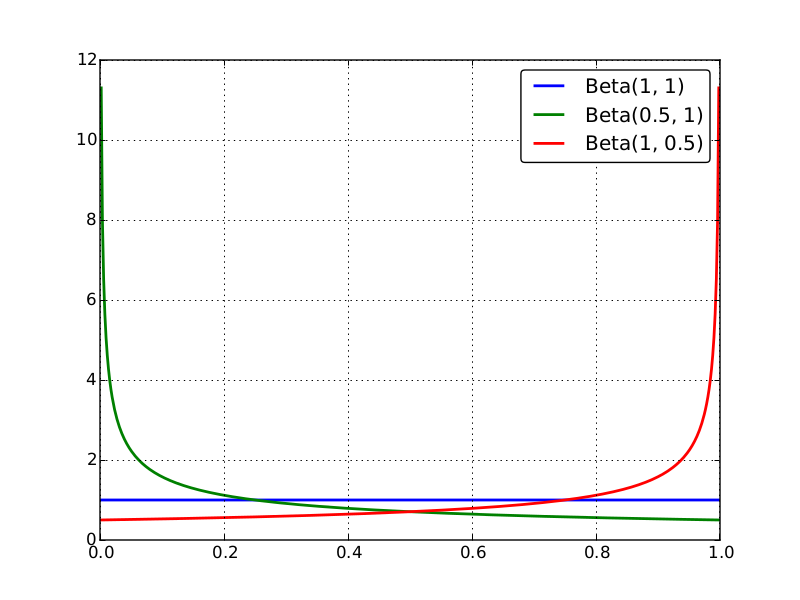
\includegraphics[width=0.7 \textwidth, keepaspectratio]{images/Beta}
  $$p(\theta|\alpha, \beta) = \frac{\theta^{\alpha-1} (1-\theta)^{\beta-1}}{B(\alpha, \beta)} \qquad B(\alpha, \beta) = \int\limits_0^1 \theta^{\alpha-1} (1-\theta)^{\beta-1} d\theta$$
\end{frame}

\begin{frame}{И снова про аддитивное сглаживание}
  Бета-распределение является априорным сопряжённым для распределения Бернулли\\  
  \begin{equation*}
    \begin{split}
    p(\theta | x, \alpha, \beta) & \propto p(\theta|\alpha, \beta) p(x|\theta) \\
      & \propto (\theta^{\alpha-1} (1-\theta)^{\beta-1})(\theta^x (1-\theta)^{1-x}) \\
      & \propto \theta^{(\alpha+x)-1} (1-\theta)^{\beta+1-x}-1 = Beta(\theta| \alpha^*, \beta^*)
    \end{split}
  \end{equation*}
\end{frame}

\begin{frame}{Оценка параметра $\theta$}
  \begin{equation*}
    \begin{split}
      \hat{\theta} &= \int\limits_{0}^1 \theta p(\theta|x, \alpha, \beta) d\theta  = \mathbb{E} [Beta(\theta|\alpha^*, \beta^*)]\\
      & = \frac{\alpha^*}{\alpha^*+\beta^*} = \frac{\alpha+x}{\alpha + \beta + 1}
    \end{split}
  \end{equation*}\\
  Если $\alpha = \beta$, то $\hat{\theta}$ в точности совпадает со сглаженной оценкой $\hat{\theta}^*$  
\end{frame}

\begin{frame}\frametitle{Что почитать по этой лекции}
  \begin{itemize}
    \item Kevin P. Murphy "Machine Learning: A Probabilistic Perspective" Chapter 3
    \item \href{http://www.ccas.ru/voron/download/Bayes.pdf}{Воронцов "Байесовские алгоритмы классификации"}
    \item Tom Mitchell "Machine Learning" Chapter 6
  \end{itemize}
\end{frame}

\begin{frame}{На следующей лекции}
  	\begin{enumerate} [--]
		\item Перцептрон
		\item Функция потерь
		\item Препроцессинг
		\item Ошибка обобщения
	\end{enumerate}
\end{frame}

\end{document}